\documentclass[11pt]{article}

% ---------- Packages ----------
\usepackage[a4paper,margin=2.5cm]{geometry}
\usepackage{graphicx}
\usepackage{booktabs}
\usepackage{longtable}
\usepackage{array}
\usepackage{xcolor}
\usepackage{hyperref}
\usepackage{fancyhdr}
\usepackage{titlesec}
\usepackage{caption}
\usepackage{float}
\usepackage{enumitem}
\usepackage{amssymb}
\usepackage[T1]{fontenc}

% ---------- Colors ----------
\definecolor{darkblue}{RGB}{31,56,100}
\definecolor{midgray}{RGB}{90,90,90}

% ---------- Section styling ----------
% ---------- Section styling ----------
\titleformat{\section}
  {\normalfont\Large\bfseries\color{darkblue}}
  {\thesection.}{0.5em}{}

\titleformat{\subsection}
  {\normalfont\large\bfseries\color{darkblue}}
  {\thesubsection}{0.5em}{}

\titleformat{\subsubsection}
  {\normalfont\normalsize\bfseries\color{midgray}}
  {\thesubsubsection}{0.5em}{}

% Reduce spacing before and after headings
\titlespacing*{\section}{0pt}{1.2ex plus .3ex minus .2ex}{0.6ex}
\titlespacing*{\subsection}{0pt}{1.0ex plus .2ex minus .2ex}{0.4ex}
\titlespacing*{\subsubsection}{0pt}{0.7ex plus .2ex minus .1ex}{0.3ex}

% ---------- Header / Footer ----------
\pagestyle{fancy}
\fancyhf{}
\renewcommand{\headrulewidth}{0.4pt}
\fancyhead[L]{\small Group 8: Employee Attrition Report}
\fancyhead[R]{\small \thepage}
\fancyfoot[C]{\small People Analytics: Who's a Flight Risk?}

% ---------- Hyperref ----------
\hypersetup{
    colorlinks=true,
    linkcolor=darkblue,
    urlcolor=darkblue,
    citecolor=darkblue,
    pdftitle={Group 8 - Employee Attrition Report | AUCA Machine Learning},
    pdfauthor={Group 8 - MSc Big Data Analytics, AUCA},
    pdfsubject={Machine Learning - Employee Attrition Prediction and Segmentation}
}

\newcommand{\resultfigure}[3]{%
    \begin{figure}[H]
        \centering
        \includegraphics[width=#2\textwidth,height=0.82\textheight,keepaspectratio]{#1}
        \caption{#3}
    \end{figure}
}

\setlength{\parskip}{0.5em}
\setlength{\parindent}{0pt}

\begin{document}

% ===================== TITLE PAGE =====================
\begin{titlepage}
    \centering
    \vspace*{0.5cm}

    
\includegraphics[width=3.2cm]{../figures/auca_logo.png}\\[0.6cm]

    {\Large \bfseries \color{darkblue} ADVENTIST UNIVERSITY OF CENTRAL AFRICA}\\[0.2cm]
    {\large (AUCA)}\\[0.2cm]
    {\normalsize Master of Science, Big Data Analytics}\\[1.4cm]

    {\LARGE \bfseries GROUP 8}\\[0.5cm]
    {\Huge \bfseries \color{darkblue} PEOPLE ANALYTICS: \\[0.2cm] WHO'S A FLIGHT RISK?}\\[0.8cm]
    {\Large Employee Attrition Prediction and Segmentation}\\[1.4cm]

    {\large \bfseries Team Members}\\[0.4cm]
    \begin{tabular}{cll}
    \toprule
    \textbf{\#} & \textbf{Student ID} & \textbf{Full Name} \\
    \midrule
    1 & 20251MBI007 & Shimwa Uwase Sylvie \\
    2 & 20251MBI017 & Ishimwe Divin Claudel \\
    3 & 20251MBI029 & Mpayimana Iradukunda Robert \\
    4 & 20251MBI050 & Hirwa Fabrice \\
    \bottomrule
    \end{tabular}\\[1.4cm]

    \begin{tabular}{rl}
    \textbf{Course:} & Machine Learning \\
    \textbf{Lecturer:} & Dr.\ Lema Logamou Seknewna \\
    \end{tabular}\\[1.2cm]

    {\large \bfseries FINAL PROJECT REPORT}\\[0.4cm]
    {\large September 2026}
    \vfill
\end{titlepage}

% ===================== TOC =====================
\tableofcontents
\newpage

% ===================== SECTION 1 =====================
\section{Executive Summary}

Employee attrition is an important people-analytics problem because organisations need to understand patterns associated with employees leaving and identify opportunities for earlier retention interventions. This project investigates employee attrition using exploratory data analysis, unsupervised learning and supervised machine learning.

The analysis was conducted on a dataset containing 1,470 employee records and 35 original variables. Data preparation included checks for missing values, duplicate records, constant variables, identification and removal of the employee identifier, investigation of potential outliers, and categorical encoding. The \texttt{EmployeeNumber} identifier was removed because it does not represent a meaningful employee characteristic for prediction. The final cleaned dataset contained 1,470 employees and 31 columns before categorical encoding.

The exploratory analysis showed that attrition is an imbalanced outcome. 1,233 employees (83.88\%) stayed, while 237 employees (16.12\%) left. This imbalance was taken into account throughout the supervised-learning stage rather than relying on accuracy alone.

The unsupervised analysis used 11 employee characteristics covering engagement, satisfaction, workload and tenure. PCA was used to examine the main dimensions of variation, while K-Means was evaluated across different values of $K$ using WCSS/inertia and silhouette scores. $K=2$ was selected because it produced the highest silhouette score of 0.2176. The resulting personas were primarily distinguished by tenure and professional experience. The early-tenure persona contained 957 employees (65.1\%) and had an observed attrition rate of 18.81\%, compared with 11.11\% among the 513 employees in the experienced long-tenure persona.

For supervised learning, three classification algorithms were compared: Logistic Regression, Support Vector Machine (SVM), and Random Forest. Class imbalance was addressed using class weighting, and model development used stratified cross-validation and hyperparameter tuning. Performance was evaluated using precision, recall, F1-score and PR-AUC, with particular emphasis on F1-score because of the minority attrition class.

The SVM was selected as the final model because it achieved the highest test-set F1-score of 0.519, with a recall of 0.596, precision of 0.459, accuracy of 0.823, and PR-AUC of 0.569. Logistic Regression achieved a higher PR-AUC of 0.624, but its F1-score was lower at 0.489. Random Forest achieved an F1-score of 0.386. Therefore, SVM provided the strongest balance between precision and recall for the project's stated objective.

SHAP was then used to interpret the final SVM. At the global level, \texttt{OverTime} had the strongest influence on the model's attrition predictions, followed by \texttt{StockOptionLevel}, \texttt{Age}, \texttt{EnvironmentSatisfaction} and \texttt{TotalWorkingYears}. The SHAP analysis describes how features contribute to model predictions and does not establish causal relationships.

At the individual level, the model was used to explain the prediction for Employee 357. The employee had an actual outcome of \textit{Left}, and the SVM predicted \textit{Left} with a 93.1\% probability. The individual SHAP analysis identified \texttt{OverTime}, \texttt{Age}, \texttt{EnvironmentSatisfaction}, \texttt{TotalWorkingYears} and \texttt{BusinessTravel} among the strongest contributors to the prediction.

Overall, the findings show that machine learning can provide useful predictive and descriptive insights into employee attrition. However, the results should be treated as decision-support information rather than causal evidence or an automatic basis for HR decisions. The model should support further investigation and appropriate human judgement rather than automatically labelling employees as flight risks.

% ===================== SECTION 2 =====================
\section{Problem Framing and Business Question}

\subsection{Business Problem}

Employee turnover can create operational disruption, recruitment costs, loss of organisational knowledge and additional pressure on remaining employees. From an HR perspective, understanding which employee characteristics are associated with attrition can help identify areas where retention strategies may be appropriate.

The project therefore focuses on the following question:

\begin{quote}
\itshape Which employee characteristics and employee segments are associated with attrition, and can supervised machine-learning models provide useful predictions of whether an employee is likely to leave?
\end{quote}

\subsection{Analytical Objectives}

The project has four main objectives:

\begin{enumerate}[label=(\arabic*)]
    \item Examine the structure and quality of the employee dataset.
    \item Identify important patterns associated with employee attrition through EDA.
    \item Develop employee personas using PCA and K-Means and examine their observed attrition rates.
    \item Develop and compare at least three supervised classification models while appropriately handling class imbalance and explaining predictions using SHAP.
\end{enumerate}

% ===================== SECTION 3 =====================
\section{Dataset and Data Preparation}

\subsection{Dataset Overview}

The original dataset contains 1,470 employee records and 35 variables. The variables describe different aspects of employees, including demographic characteristics, job information, satisfaction, compensation, workload, performance and organisational tenure.

The target variable for supervised learning is \texttt{Attrition}, which indicates whether the employee left the organisation.

\begin{table}[H]
\centering
\begin{tabular}{lrr}
\toprule
\textbf{Attrition} & \textbf{Employees} & \textbf{Percentage} \\
\midrule
Stayed (0) & 1,233 & 83.88\% \\
Left (1)   & 237   & 16.12\% \\
\midrule
Total      & 1,470 & 100\% \\
\bottomrule
\end{tabular}
\caption{Target variable distribution}
\end{table}

The relatively small proportion of employees who left demonstrates why class imbalance is an important consideration in the predictive modelling stage.

\subsection{Data Cleaning}

\subsubsection*{Missing values}
The dataset was checked for missing values. The supervised-learning target contained no missing values.

\subsubsection*{Duplicate records}
The dataset contained zero duplicate rows, so no observations needed to be removed for duplication.

\subsubsection*{Constant variables}
Variables containing only one unique value were identified because they provide no useful information for prediction or clustering.

\subsubsection*{Identifier removal}
\texttt{EmployeeNumber} was removed because it is an identifier rather than a meaningful employee characteristic. After removing constant and identifier columns, the dataset contained 1,470 rows and 31 columns.

\subsubsection*{Outlier investigation}
Potential outliers were investigated using boxplots and the IQR method. Outliers were not automatically removed simply because they were statistically extreme. Some extreme values can represent legitimate employee characteristics.

\subsubsection*{Encoding}
Categorical variables were encoded for machine-learning use. The final encoded dataset contained 45 columns.

For supervised modelling, preprocessing was incorporated into machine-learning pipelines so that transformations were fitted using the training data rather than the entire dataset. This reduces the risk of data leakage.


% ===================== SECTION 4 =====================
\section{Exploratory Data Analysis}

\subsection{Attrition Distribution}

The target distribution demonstrates substantial class imbalance: 83.88\% of employees stayed and 16.12\% of employees left. This finding influenced the supervised-learning methodology. Accuracy alone could be misleading because a model could achieve relatively high accuracy by mostly predicting the majority class.

\resultfigure{../figures/fig_attrition_dist.png}{0.6}{Employee attrition distribution (Stayed vs.\ Left).}

\subsection{Relationship with Employee Characteristics}

The EDA examined both categorical and numerical employee characteristics in relation to attrition.

The correlation analysis identified \texttt{OverTime} as the strongest positive correlation with the attrition target, with a correlation of approximately 0.246. Other notable relationships included \texttt{MaritalStatus\_Single}, \texttt{TotalWorkingYears}, \texttt{JobLevel}, \texttt{YearsInCurrentRole}, \texttt{MonthlyIncome} and \texttt{Age}.

These findings provided useful direction for later modelling and interpretation, while correlation was treated as an association rather than evidence of causation.

\resultfigure{../figures/fig_correlation_heatmap.png}{0.85}{Correlation heatmap of the top features most associated with attrition.}


% ===================== SECTION 5 =====================
\section{Unsupervised Learning}

\subsection{Employee Persona Construction}

The clustering analysis was designed around the Group 8 requirement to identify employee personas based on:

\begin{itemize}
    \item \textbf{Engagement:} \texttt{JobInvolvement}
    \item \textbf{Satisfaction:} \texttt{JobSatisfaction}, \texttt{EnvironmentSatisfaction}, \texttt{RelationshipSatisfaction}, \texttt{WorkLifeBalance}
    \item \textbf{Workload:} \texttt{OverTime}
    \item \textbf{Tenure:} \texttt{TotalWorkingYears}, \texttt{YearsAtCompany}, \texttt{YearsInCurrentRole}, \texttt{YearsSinceLastPromotion}, \texttt{YearsWithCurrManager}
\end{itemize}

\texttt{Attrition} was deliberately excluded from the clustering features so that the employee personas were created independently of the outcome. The 11 selected variables were standardised before PCA and K-Means.


\subsection{PCA}

PCA was used to reduce dimensionality and identify major dimensions of variation. The first seven principal components explained 85.39\% of the total variance, while the first two components explained 40.67\%.

The first principal component was mainly associated with tenure and organisational experience, with the largest loadings coming from \texttt{YearsAtCompany} (0.505), \texttt{YearsInCurrentRole} (0.468), \texttt{YearsWithCurrManager} (0.464), \texttt{YearsSinceLastPromotion} (0.404) and \texttt{TotalWorkingYears} (0.382).

The second component was primarily associated with workload and workplace satisfaction. \texttt{OverTime} had the strongest contribution at 0.688, followed by \texttt{EnvironmentSatisfaction} at 0.560 and \texttt{RelationshipSatisfaction} at 0.449.

These component interpretations describe associations in the reduced feature space and should not be interpreted as causal relationships.

\begin{figure}[H]
    \centering
    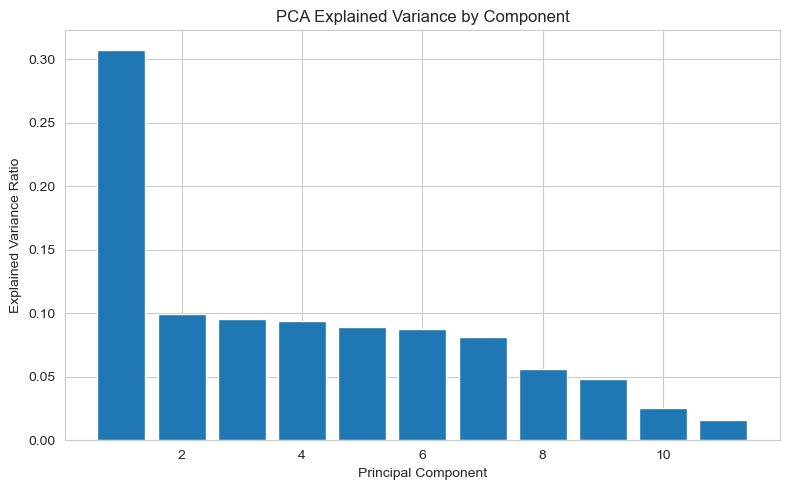
\includegraphics[width=0.48\textwidth]{../figures/fig_pca_variance.png}
    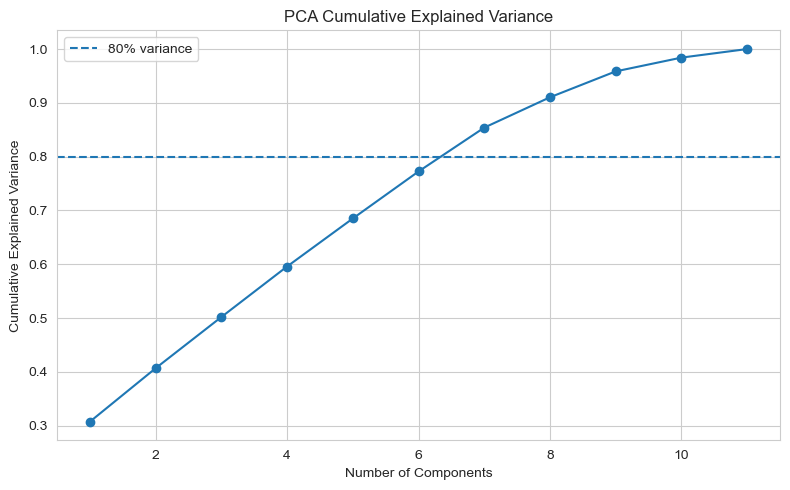
\includegraphics[width=0.48\textwidth]{../figures/fig_pca_cumulative.png}
    \caption{PCA explained variance by component (left) and cumulative explained variance (right).}
\end{figure}


\subsection{K-Means Clustering}

K-Means solutions from $K=2$ to $K=8$ were evaluated using WCSS/inertia and silhouette scores.

\begin{center}
\textbf{K=2 $\rightarrow$ Highest silhouette score = 0.2176}
\end{center}

Although the score is relatively low, $K=2$ provided the strongest separation among the tested solutions. Therefore, two employee personas were retained.

The relatively low silhouette score also means the personas should be viewed as broad employee segments rather than completely distinct employee types.

\begin{figure}[H]
    \centering
    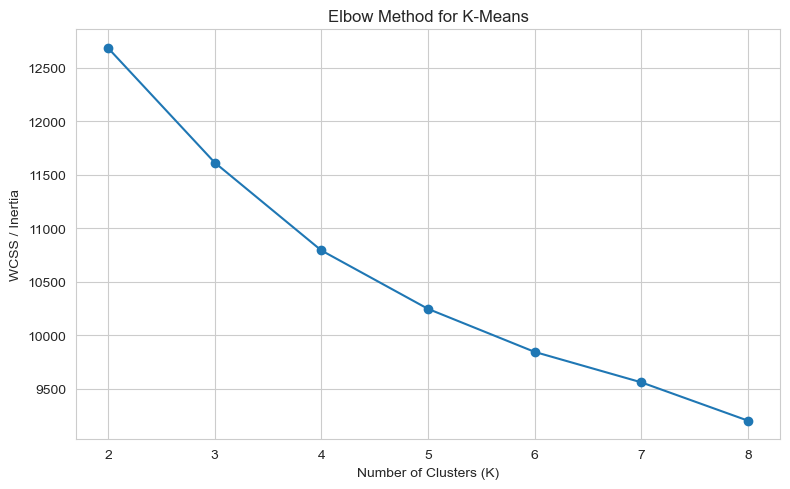
\includegraphics[width=0.48\textwidth]{../figures/fig_elbow.png}
    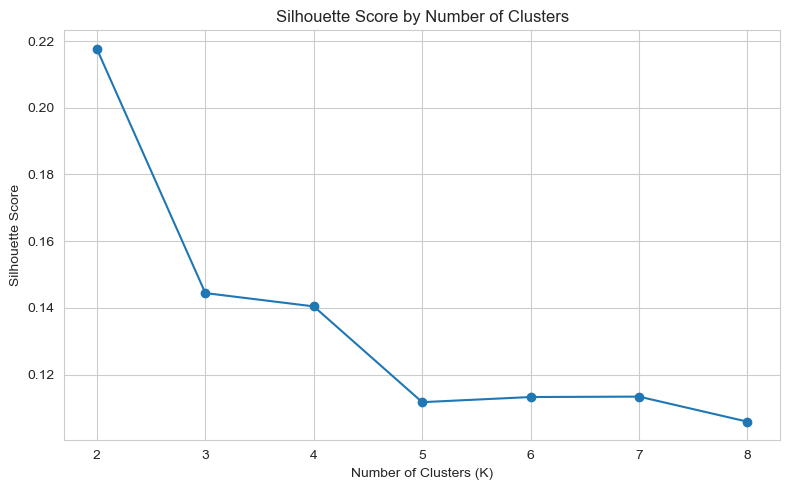
\includegraphics[width=0.48\textwidth]{../figures/fig_silhouette.png}
    \caption{Elbow method (left) and silhouette score (right) across candidate values of $K$.}
\end{figure}



\subsection{Employee Personas}

\subsubsection*{Persona 1 --- Early-Tenure Employees}

\begin{table}[H]
\centering
\begin{tabular}{lr}
\toprule
\textbf{Measure} & \textbf{Result} \\
\midrule
Employees & 957 \\
Percentage & 65.1\% \\
Average TotalWorkingYears & 8.56 \\
Average YearsAtCompany & 3.73 \\
Observed attrition rate & 18.81\% \\
\bottomrule
\end{tabular}
\caption{Persona 1 -- Early-Tenure Employees}
\end{table}

This group is characterised primarily by lower organisational and professional tenure.

\subsubsection*{Persona 2 --- Experienced Long-Tenure Employees}

\begin{table}[H]
\centering
\begin{tabular}{lr}
\toprule
\textbf{Measure} & \textbf{Result} \\
\midrule
Employees & 513 \\
Percentage & 34.9\% \\
Average TotalWorkingYears & 16.35 \\
Average YearsAtCompany & 13.13 \\
Observed attrition rate & 11.11\% \\
\bottomrule
\end{tabular}
\caption{Persona 2 -- Experienced Long-Tenure Employees}
\end{table}

This group has substantially longer organisational and professional tenure.

The clustering results indicate that tenure and professional experience are the main characteristics distinguishing the two personas, while satisfaction and engagement measures are relatively similar across the groups.

\resultfigure{../figures/fig_clusters_pca.png}{0.6}{Final K-Means clusters visualised on the first two PCA components.}

\subsection{Personas and Attrition}

The early-tenure persona has an observed attrition rate of 18.81\%, compared with 11.11\% for the experienced long-tenure persona. This represents a difference of approximately 7.70 percentage points.

The result suggests that the early-tenure segment has a higher observed level of attrition in this dataset. However, the clustering analysis is descriptive and does not establish that shorter tenure causes employees to leave.

% ===================== SECTION 6 =====================
\section{Supervised Learning}

\subsection{Modelling Strategy}

The supervised-learning task was formulated as binary classification: $0 = $ Stayed and $1 = $ Left.

The dataset was divided into 80\% training data and 20\% test data. A stratified split was used to preserve the class proportions.

The test set was kept separate from preprocessing, cross-validation and hyperparameter tuning so that it could provide an independent evaluation of model performance.


\subsection{Handling Class Imbalance}

Because only 16.12\% of employees belong to the attrition class, class imbalance was explicitly addressed.

The models used class weighting to give greater importance to observations from the minority class during training.

Performance was therefore evaluated using precision, recall, F1-score and PR-AUC rather than relying on accuracy alone.

\subsection{Models Compared}

Three supervised classification models were developed:

\begin{itemize}
    \item Logistic Regression
    \item Support Vector Machine (SVM)
    \item Random Forest
\end{itemize}

Each model was incorporated into a preprocessing pipeline, and hyperparameters were tuned using stratified five-fold cross-validation.



\subsection{Model Performance}

\begin{table}[H]
\centering
\begin{tabular}{lrrrrr}
\toprule
\textbf{Model} & \textbf{Accuracy} & \textbf{Precision} & \textbf{Recall} & \textbf{F1} & \textbf{PR-AUC} \\
\midrule
Logistic Regression & 0.765 & 0.375 & 0.702 & 0.489 & 0.624 \\
SVM                  & 0.823 & 0.459 & 0.596 & 0.519 & 0.569 \\
Random Forest        & 0.827 & 0.444 & 0.340 & 0.386 & 0.431 \\
\bottomrule
\end{tabular}
\caption{Test-set performance of the three candidate models}
\end{table}

The results show why accuracy alone is insufficient. Random Forest has slightly higher accuracy than SVM, but its recall and F1-score are substantially lower.

Logistic Regression has the highest PR-AUC and recall, but SVM has the highest F1-score.

\resultfigure{../figures/fig_model_comparison.png}{0.7}{Comparison of precision, recall, F1-score and PR-AUC across the three candidate models.}

\begin{figure}[H]
    \centering
    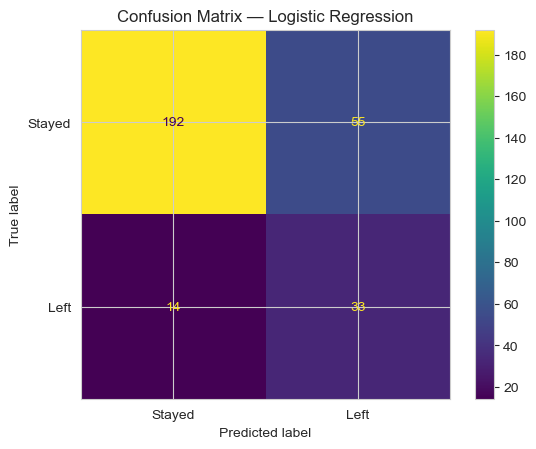
\includegraphics[width=0.32\textwidth]{../figures/fig_cm_logreg.png}
    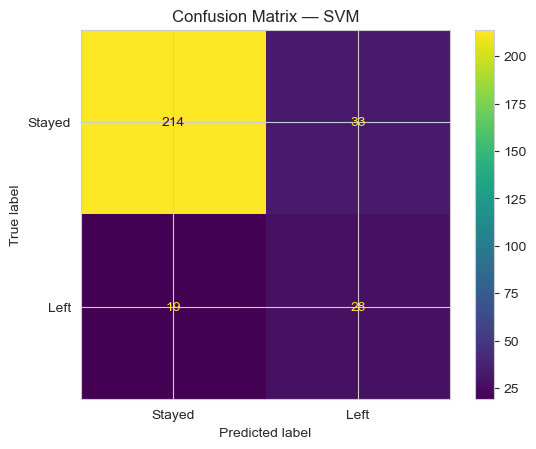
\includegraphics[width=0.32\textwidth]{../figures/fig_cm_svm.png}
    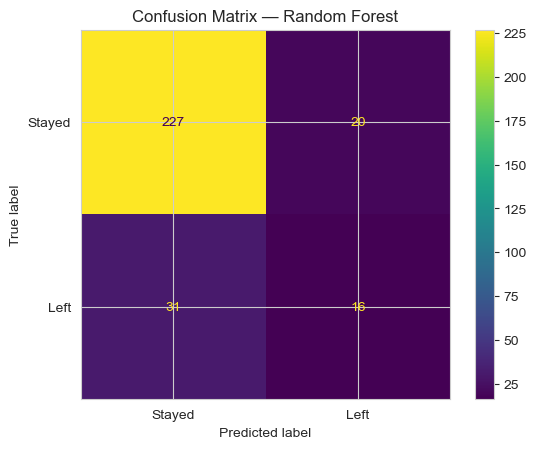
\includegraphics[width=0.32\textwidth]{../figures/fig_cm_rf.png}
    \caption{Confusion matrices on the held-out test set: Logistic Regression (left), SVM (centre), Random Forest (right).}
\end{figure}


\subsection{Final Model Selection}

\textbf{Final model: Support Vector Machine (SVM)}

SVM was selected as the final model because it achieved the highest test-set F1-score of 0.519. F1 provides a balance between precision and recall, which is appropriate for the flight-risk objective.

Although Logistic Regression achieved a higher PR-AUC of 0.624, its F1-score was lower at 0.489. Therefore, SVM was selected as the model providing the strongest balance between precision and recall according to the primary selection criterion.

\begin{table}[H]
\centering
\begin{tabular}{lr}
\toprule
\textbf{Final SVM Metric} & \textbf{Result} \\
\midrule
Accuracy & 0.823 \\
Precision & 0.459 \\
Recall & 0.596 \\
F1-score & 0.519 \\
PR-AUC & 0.569 \\
\bottomrule
\end{tabular}
\caption{Final SVM performance on the test set}
\end{table}

% ===================== SECTION 7 =====================
\section{Model Interpretation}

\subsection{Global SHAP Interpretation}

SHAP was used to interpret the selected SVM because the model does not provide tree-based feature importance.

The SHAP analysis aggregated encoded categorical variables back to their original employee-level variables to make the results easier to interpret.



\begin{table}[H]
\centering
\begin{tabular}{ll}
\toprule
\textbf{Rank} & \textbf{Feature} \\
\midrule
1  & OverTime \\
2  & StockOptionLevel \\
3  & Age \\
4  & EnvironmentSatisfaction \\
5  & TotalWorkingYears \\
6  & NumCompaniesWorked \\
7  & DistanceFromHome \\
8  & RelationshipSatisfaction \\
9  & JobInvolvement \\
10 & JobRole \\
\bottomrule
\end{tabular}
\caption{Top ten features by global SHAP importance}
\end{table}

\resultfigure{../figures/fig_shap_global.png}{0.75}{Global SHAP feature importance for the final SVM model.}

The strongest overall feature was \texttt{OverTime}, meaning it had the largest average absolute contribution to the SVM's predictions in the SHAP analysis.

Importantly, this does not mean that \texttt{OverTime} causes attrition. SHAP explains the contribution of a feature to the model's prediction, not a causal relationship.

% ===================== SECTION 8 =====================
\section{Individual Employee Explanation}

To demonstrate individual-level interpretability, the employee in the held-out test set with the highest predicted probability of attrition was selected.

\subsection*{Employee 357}

\begin{table}[H]
\centering
\begin{tabular}{lr}
\toprule
\textbf{Measure} & \textbf{Result} \\
\midrule
Actual outcome & Left \\
Predicted outcome & Left \\
Predicted probability of leaving & 93.1\% \\
\bottomrule
\end{tabular}
\caption{Employee 357 -- individual prediction summary}
\end{table}

The individual SHAP analysis identified the following major contributors:

\begin{table}[H]
\centering
\begin{tabular}{lll}
\toprule
\textbf{Feature} & \textbf{Employee Value} & \textbf{SHAP Direction} \\
\midrule
OverTime & 1 & Increases flight-risk prediction \\
Age & 21 & Increases flight-risk prediction \\
EnvironmentSatisfaction & 1 & Increases flight-risk prediction \\
TotalWorkingYears & 3 & Increases flight-risk prediction \\
BusinessTravel & Travel\_Frequently & Increases flight-risk prediction \\
JobRole & Sales Representative & Increases flight-risk prediction \\
YearsWithCurrManager & 2 & Increases flight-risk prediction \\
StockOptionLevel & 0 & Increases flight-risk prediction \\
JobInvolvement & 2 & Increases flight-risk prediction \\
MonthlyIncome & 2174 & Increases flight-risk prediction \\
\bottomrule
\end{tabular}
\caption{Individual SHAP contributors for Employee 357}
\end{table}


\resultfigure{../figures/fig_shap_waterfall.png}{0.85}{SHAP waterfall plot for Employee 357.}

The waterfall plot illustrates how the feature contributions moved the model's prediction toward the final 93.1\% probability of leaving.

Again, these are predictive contributions, not causal effects.

% ===================== SECTION 9 =====================
\section{Limitations, Ethics and HR Implications}

Several limitations should be considered when interpreting the results.

\textbf{First}, the dataset is imbalanced, with only 16.12\% of employees belonging to the attrition class. Although class weighting and appropriate evaluation metrics were used, minority-class prediction remains challenging.

\textbf{Second}, the SVM achieved an F1-score of 0.519 and recall of 0.596. This means that the model does not identify every employee who leaves and will also produce false positive risk predictions.

\textbf{Third}, the clustering silhouette score of 0.2176 indicates relatively weak separation between the two personas. The clusters should therefore be treated as broad descriptive segments rather than sharply separated employee types.

\textbf{Fourth}, SHAP values explain model behaviour but do not demonstrate causation. For example, the finding that \texttt{OverTime} had the strongest influence on the SVM's predictions should not be interpreted as proof that overtime causes employees to leave.

From an HR perspective, the model should therefore be used as an early-warning and decision-support tool. It should not automatically label employees as flight risks or be used as the sole basis for employment decisions. Any intervention should consider the employee's broader context and involve appropriate human judgement.

% ===================== SECTION 10 =====================
\section{Conclusion}

This project combined exploratory analysis, employee segmentation and supervised machine learning to investigate employee attrition.

The unsupervised analysis identified two broad employee personas primarily differentiated by organisational and professional tenure. The early-tenure group represented 65.1\% of employees and had a higher observed attrition rate of 18.81\%, compared with 11.11\% for the experienced long-tenure group.

The supervised analysis compared Logistic Regression, SVM and Random Forest while explicitly addressing class imbalance. SVM was selected as the final model because it achieved the highest test-set F1-score of 0.519, providing the strongest balance between precision and recall according to the project's selection criterion.

SHAP interpretation showed that \texttt{OverTime} had the strongest overall influence on the SVM's attrition predictions. The individual explanation demonstrated that Employee 357 received a 93.1\% predicted probability of leaving and was actually recorded as having left.

Overall, the analysis demonstrates the potential of machine learning to provide useful insights and early-warning information for employee attrition. However, the results should be used to support further HR investigation and retention planning rather than to make automatic decisions about individual employees.

% ===================== REFERENCES =====================
\newpage
\section*{References}
\addcontentsline{toc}{section}{References}

\subsection*{Course Activity Notebooks}

\begin{enumerate}[label=\arabic*.]
    \item \texttt{01\_Logistic\_Regression.ipynb}. Course practical activity on Logistic Regression.
    \item \texttt{03\_SVM.ipynb}. Course practical activity on Support Vector Machines (SVM).
    \item \texttt{05\_Random\_Forest.ipynb}. Course practical activity on Random Forest classification and feature importance.
    \item \texttt{06\_XGBoost.ipynb}. Course practical activity on XGBoost and model interpretation using SHAP.
    \item \texttt{07\_Model\_Comparison\_Dashboard.ipynb}. Course practical activity on machine learning model comparison and evaluation.
    \item \texttt{08\_KMeans\_Clustering.ipynb}. Course practical activity on K-Means clustering.
    \item \texttt{11\_PCA.ipynb}. Course practical activity on Principal Component Analysis (PCA).
\end{enumerate}

\subsection*{AI Assistance}

OpenAI. \textit{ChatGPT}. Used as an AI-assisted learning and support tool to explain machine learning concepts, clarify course activities, interpret errors, explain code, and provide guidance during the development and interpretation of the project. The final analysis, implementation, results, and conclusions were reviewed and adapted by the project team.


% ===================== TEAM CONTRIBUTIONS =====================
\section*{Team Contributions}
\addcontentsline{toc}{section}{Team Contributions}

\begin{table}[H]
\centering
\begin{tabular}{p{0.38\textwidth}p{0.55\textwidth}}
\toprule
\textbf{Member} & \textbf{Role} \\
\midrule
Mpayimana Iradukunda Robert & Data \& Cleaning Lead \\
\addlinespace
Ishimwe Divin Claudel & Unsupervised Learning Lead \\
\addlinespace
Shimwa Uwase Sylvie & Supervised Learning Lead \\
\addlinespace
Hirwa Fabrice (Rugera) & Story \& Interpretation Lead --- SHAP, report, slides \\
\bottomrule
\end{tabular}
\caption{Group 8 contributions by member}
\end{table}

\begin{center}
    \vspace{1cm}
    \textbf{Thank You}
\end{center}

\end{document}
